% Тут используется класс, установленный на сервере Papeeria. На случай, если
% текст понадобится редактировать где-то в другом месте, рядом лежит файл matmex-diploma-custom.cls
% который в момент своего создания был идентичен классу, установленному на сервере.
% Для того, чтобы им воспользоваться, замените matmex-diploma на matmex-diploma-custom
% Если вы работаете исключительно в Papeeria то мы настоятельно рекомендуем пользоваться
% классом matmex-diploma, поскольку он будет автоматически обновляться по мере внесения корректив
%

% По умолчанию используется шрифт 14 размера. Если нужен 12-й шрифт, уберите опцию [14pt]
%\documentclass[14pt]{matmex-diploma}
\documentclass[14pt]{matmex-diploma-custom}
\usepackage{graphicx}
\usepackage{float}
\usepackage{cite}
\usepackage{amsmath,amssymb,amsfonts}
\usepackage{caption}
\usepackage{textcomp}
\usepackage{xcolor}
\usepackage{float}
\usepackage{amssymb}
\usepackage{makecell}
\usepackage[mathscr]{euscript}

\usepackage{indentfirst}



\newcommand\name[1]{\textsc{#1}}

\begin{document}
% Год, город, название университета и факультета предопределены,
% но можно и поменять.
% Если англоязычная титульная страница не нужна, то ее можно просто удалить.
\filltitle{ru}{
    chair              = {Программная инженерия},
    title              = {Декларативный предметно-ориентированный язык разработки мобильных приложений},
    type               = {diploma},
    position           = {студента},
    group              = 671,
    author             = {Поляков Александр Романович},
    supervisorPosition = {старший преподаватель},
    supervisor         = {Дмитрий Вадимович Луцив},
    reviewerPosition   = {руководитель направления разработки языков\\Huawei R\&D},
    reviewer           = {Алексей Евгеньевич Недоря}
%   university         = {Санкт-Петербургский Государственный Университет},
%   faculty            = {Математико-механический факультет},
%   city               = {Санкт-Петербург},
%   year               = {2019}
}
% \filltitle{en}{
%     chair              = {Software Engineering},
%     title              = {Automated compiler optimizations tuning},
%     author             = {Alexander Polyakov},
%     supervisorPosition = {},
%     supervisor         = {},
%     reviewerPosition   = {},
%     reviewer           = {},
% }
\maketitle
\tableofcontents
% У введения нет номера главы
\section*{Введение}
Жизнь человека в настоящее время тяжело представить без носимых устройств,
проникших практически во все сферы деятельности оного.
Человеко-машинное взаимодействие в данном случае в большинстве своём
осуществляется посредством мобильных приложений -- программного обеспечения, специально разработанного для запуска на мобильных устройствах, таких как
смартфоны, планшеты, умные часы, автомобили.
Изобилие устройств повлекло за собой разнообразие архитектур
процессоров~\cite{cpu-arches, mobile-phones-cpu-trends} и операционных систем, которые необходимо учитывать при разработке приложения.

Несмотря на то, что в создании современных мобильных приложений явно
прослеживается тренд на унификацию методологий, интерфейсов, компонентов и других атрибутов разработки программного обеспечения, своеобразными
аттракторами данной унификации стали пара наиболее популярных мобильных операционных систем вкупе с несколькими схожими архитектурами процессоров. 
Перенос программного обеспечения на другие платформы до сих пор остаётся одним
из основных подходов к разработке мультиплатформенных мобильных
приложений~\cite{mob-apps-approaches}.
В последнее время набирают популярность средства разработки программного
обеспечения~\cite{kotlin-homepage,swift-homepage,flutter-homepage,
reactnative-homepage, vuenative-homepage}, позволяющие разработчикам работать
над единой кодовой базой приложения, предназначенной для работы с несколькими
конфигурациями пользовательских устройств.

Одним из важных требований к современным средствам разработки
мультиплатформенных мобильных приложений является возможность декларативного
описания пользовательского интерфейса.
Такая возможность позволяет ускорить и удешевить разработку мобильных
приложений за счёт разделения труда между программистами логики приложения и
дизайнерами пользовательского интерфейса, сохранив при этом единство окружения
разработки и исполнения.
Современным и популярным подходом к предоставлению пользователям данной
функциональности является использование декларативных
предметно-ориентированных языков -- языков программирования с высоким уровнем
абстракции, отражающих специфику решаемых с их помощью задач, оперируя понятиями и правилами из определённой области.

\name{Accord} -- язык программирования общего назначения, зародившийся и
разрабатываемый в российском научно-исследовательском институте компании
\name{Huawei} и находящийся на данный момент в стадии ранней разработки.
Одной из наиболее перспективных ниш для данного языка является разработка
мобильных приложений, требующая от языка, как было описано выше, возможности
декларативного описания интерфейсов мультиплатформенных приложений.
\section{Постановка задачи}
Целью данной работы является создание языка разработки
мобильных приложений, основанного на языке программирования общего
назначения \name{Accord}. Для её достижения были поставлены следующие задачи:
\begin{itemize}
	\item выполнить сбор и анализ требований к современному языку
	разработки мобильных приложений;
	\item выполнить обзор предметной области и существующих решений;
	\item предложить подход к созданию языка разработки мобильных
	приложений, удовлетворяющему собранным требованиям;
	\item реализовать данный язык;
	\item провести его апробацию.
\end{itemize}
\section{Требования к спецификации и компилятору языка разработки мобильных приложений}
\label{requirements-section}
В данном разделе представлены требования к современному средству
разработки мобильных приложений, собранные на основе обзора существующих
решений, а также сводная таблица соответствия существующих решений собранным
требованиям. Предъявляемые требования были разделены на две группы:
функциональные и нефункциональные.


\subsection{Функциональные требования}
\subsubsection*{Оптимизация отрисовки графического интерфейса во время компиляции мобильного приложения}
Отрисовка графического интерфейса мобильного приложения является
ресурсоёмкой задачей. Так, для современного мобильного устройства,
обладающего следующими характеристиками:
\begin{itemize}
	\item разрешение экрана $1644 \times 3840$ точек;
	\item обновление кадра с частотой $120$ Гц;
\end{itemize}
пропускная способность графического конвейера, при условии хранения цвета
одного пикселя в четырёх байтах, должна составлять\\$1644 * 3840 * 4 * 120 = 3030220800$
байт в секунду, что составляет около $2.8$ гигабайт. Такая
нагрузка на мобильное устройство недопустима ввиду скромных возможностей
охлаждения таких устройств, а также ввиду ограниченного объема заряда
аккумуляторной батареи.

Более того, при условии необходимости обновления кадров с частотой $120$ Гц,
новый кадр должен быть доставлен движку отрисовки не позднее, чем через
$8$ мс после отрисовки предыдущего. Если флагманские мобильные устройства
и способны обеспечить должную производительность классического подхода к
обновлению интерфейса, представленного в пункте~\ref{section:render-pipeline},
за счёт увеличенного энергопотребления, то менее мощные устройства на это
уже не способны.

Исходя из вышеописанного, становится очевидной важность
различных оптимизаций отрисовки интерфейса. В особенности тех, что
могут быть применены во время компиляции приложения.

\subsubsection*{Реактивные обновления пользовательского интерфейса}
Реактивное программирование --- парадигма программирования, ориентированная
на потоки данных и распространение изменений. Это означает cуществование
возможности выражения статических и динамических потоков данных, а также то,
что нижележащая модель исполнения должна автоматически распространять
изменения благодаря в рамках определённого потока данных. В контексте
разработки графического интерфейса, под реактивностью понимается
автоматическое обновление пользовательского интерфейса при изменении
данных, помеченных как реактивные.

\subsection{Нефункциональные требования}
\subsubsection*{Декларативность описания пользовательского интерфейса мобильного приложения}
В отличие от императивного программирования интерфейсов, в котором
разработчик задаёт как именно необходимо построить интерфейс, декларативное
описание интерфейсов позволяет разработчику указать то, что он хочет увидеть
на экране, не заботясь о том, каким образом интерфейс будет построен.

\subsubsection*{Предоставление отладочных возможностей}
Отладка программ --- неизбежный процесс, возникающий при разработке
большого и сложного программного обеспечения. Существуют несколько видов
отладки: отладочный вывод, трассировка, использование отладчика.
Наиболее совершенным способом отладки является применение
специальных инструментов --- отладчиков. Однако, несмотря на это,
существуют ситуации, когда использование отладчика невозможно по каким-либо
причинам. Поэтому современный язык разработки мобильных приложений должен
предоставлять пользователям различные виды отладки для решения разного
спектра проблем.

\subsubsection*{Кроссплатформенная разработка}
Возможность разработки и поддержки единой кодовой базы мобильного приложения
уже многие годы является потребностью разработчиков. Такая возможность
сказывается на стоимости разработки приложения, что, в свою очередь,
через стоимость конечного продукта влияет и на пользовательский опыт,
получаемый потребителем от взаимодействия с приложением.

\subsubsection*{Поддержка интегрированной средой разработки}
Интегрированная среда разработки стала неотъемлемой частью процесса
разработки комплексных программных систем. Мобильный приложения являются
примерами таких систем, поскольку зачастую при их разработке требуется
не только окружение для работы с исходным кодом, но и для работы с
ресурсами приложения, базой данных и так далее.


\subsection{Соответствие существующих решений собранным требованиям}
В таблице~\ref{existing-solutions-table} отображено соответствие
популярных существующих решений собранным требованиям к языку разработки
мобильных приложений и его компилятору. Как видно из таблицы, ни одно
из существующих решений не соответствует всем собранным в данной работе
требованиям.
\begin{table}[h]
	\begin{tabular}{|c|c|c|c|c|}
		\hline
		
		& \thead{Dart/\\Flutter} & \thead{Kotlin\\UI DSL} &
		 \thead{React\\Native} & \thead{Swift/\\SwiftUI} \\
		
		\hline
		\makecell{Оптимизация отрисовки\\графического интерфейса\\
		во время компиляции\\мобильного приложения}
		& -- & -- & -- & + \\
		
		\hline
		\makecell{Реактивные обновления\\пользовательского интерфейса}
		& + & + & + & + \\
		
		\hline
		\makecell{Декларативность описания\\пользовательского интерфейса}
		& + & + & + & + \\
		
		\hline
		\makecell{Кроссплатформенная разработка}
		& + & + & + & -- \\
		
		\hline
		\makecell{Предоставление отладочных\\возможностей}
		& + & + & + & + \\
		
		\hline
		\makecell{Поддержка интегрированной\\средой разработки}
		& + & + & + & + \\
		
		\hline
        \end{tabular}
        \caption{Сводная таблица соответствия существующих решений собранным требованиям}
        \label{existing-solutions-table}
\end{table}

\section{Обзор}
В данном разделе представлен обзор предметной области:
основные способы реализации предметно-ориентированных языков; 
процесс отображения пользовательских интерфейсов;
существующие языки программирования общего назначения, предоставляющие
пользователям возможность декларативного описания пользовательских
интерфейсов с помощью предметно-ориентированных языков.

\subsection{Предметная область}
\subsubsection{Предметно-ориентированные языки}
Предметно-ориентированный язык (\textit{domain-specific language}, DSL) ---
это язык программирования с более высоким уровнем абстракции,
отражающий специфику решаемых с его помощью задач. Такой язык оперирует
понятиями и правилами из определенной предметной области~\cite{book-of-dsls}.

В отличие от языков программирования общего назначения, таких как \name{C},
\name{Python}, \name{Java}, предметно-ориентированные языки предоставляют
абстракции, адекватные решаемой проблеме, позволяя выражать решения,
написанные с их помощью, кратко и ёмко; причём в некоторых случаях
использование DSL не требует квалификации программиста.
В качестве примера DSL можно привести \name{SQL} ---  декларативный язык
программирования, применяемый для создания, модификации и управления данными в
реляционной базе данных.
Основным недостатком применения предметно-ориентированных языков является
стоимость их разработки, требующая экспертизы как в области разработки языков
программирования, так и в целевой предметной области.
Это является одной из причин того, что предметные языки редко применяются
для решения задач программной инженерии, в отличие от языков программирования
общего назначения.
Другой причиной отказа от обособленных предметных языков является тот факт,
что сочетание программной библиотеки и языка программирования общего
назначения может заменять DSL.
Программный интерфейс (\textit{Application Programming Interface},
API) библиотеки содержит специфичный для определённой
области словарь, образованный именами классов, методов и функций, доступный
всем пользователям языков программирования общего назначения, подключившим
библиотеку.
Однако, вышеприведённый подход проигрывает предметным языкам в следующих
аспектах~\cite{when-and-how-develop-dsl,dsl-spectrum-wile}:
\begin{itemize}
	\item устоявшаяся в области нотация, как правило, выходит за рамки
	ограниченных механизмов определения пользовательских операторов,
	предоставляемых языками общего назначения;
	\item абстракции определённой области не всегда могут быть
	просто отображены в конструкции языков общего назначения~\cite{dsl-traversal-transform};
	\item использование предметно-ориентированного языка сохраняет
	возможность анализа, верификации, оптимизации, параллелизации и
	трансформации в рамках конкретной области, что, в случае работы с
	исходным текстом языка программирования общего назначения, является
	более сложной задачей.
\end{itemize}

\subsubsection{Подходы к реализации предметно-ориентированных языков}
В последнее время всё больше исследований в области
предметно-ориен\-тированных языков направлены на категоризацию предметных
языков, а также выработку советов и лучших практик, отвечающих на вопросы
"когда и как?" создавать DSL для конкретной области~\cite{when-and-how-develop-dsl,study-on-preliminary-approaches-develop-dsl,spinellis-dsl-patterns}.
\paragraph{Препроцессинг}
DSL-конструкции транслируются в более низкоуровневый программный код
базового языка программирования общего назначения.
\begin{itemize}
	\item \textit{Макрокоманда}. Конструкции предметного языка представлены
	символьными именами, заменяемыми при обработке препроцессором на
	последовательность программных инструкций базового языка.
	\item \textit{Транспиляция}. Исходный код предметного языка
	транслируется в исходный код языка общего назначения.
	\item \textit{Лексическая обработка}. Трансформация предметного языка в
	язык общего назначения осуществляется на уровне лексем.
\end{itemize}

Преимуществом данного подхода является простота реализации DSL, поскольку
большая часть семантического анализа выполняется средствами базового языка.
В то же время, это является и недостатком данного подхода ввиду отсутствия
предметно-ориентированного статического анализа, оптимизаций и сообщений об ошибках.

\paragraph{Встраивание в базовый язык}
В данном подходе конструкции базового языка используются для построения
библиотеки предметно-ориен\-тированных операций. С помощью синтаксиса
базового языка задаётся диалект, максимально приближенный к определённой
предметной области.

Преимуществом данного подхода является полное переиспользование компилятора или интерпретатора базового языка для построения DSL. Основными недостатками
являются сообщения об ошибках, соответствующие спецификации базового языка,
и ограниченная синтаксическая выразительность, обусловленная
существующим синтаксисом базового языка.

\paragraph{Самостоятельный компилятор}
В данном подходе для создания DSL используются методы построения
компиляторов или интерпретаторов. В случае компилятора, конструкции
предметного языка транслируются во внутреннее представление компилятора, а
статический анализ производится над спецификацией DSL. В случае
интерпретатора, конструкции предметного языка распознаются и выполняются
в ходе цикла выборки-распознавания-исполнения (fetch-decode-execute cycle).

Преимуществами данного подхода являются приближенные к предметной
области синтаксис языка и сообщения об ошибках. Серьёзным недостатком
является необходимость создания нового компилятора или интерпретатора
предметного языка.

\paragraph{Компилятор компиляторов}
Данный подход схож с предыдущим за исключением того, что все или некоторые
стадии компиляции выполняются с использованием \textit{компилятора компиляторов} --- программы, воспринимающей синтаксическое или семантическое
описание языка программирования и генерирующей компилятор для этого языка.

Преимуществом подхода является снижение расходов на создание компилятора
предметного языка. Ограниченность итогового DSL возможностями используемого
компилятора компиляторов, а также сложность проработки предметного языка в
деталях, что может быть критично для достижения определённого уровня
производительности и близости сообщений об ошибках к предметной области,
составляют недостатки данного подхода.

\paragraph{Расширение существующего компилятора}
Компилятор языка программирования общего назначения расширяется
предметно-ориенти\-рованными правилами оптимизации и/или генерации кода.

В сравнении с предыдущим, данный подход менее трудоёмок из-за возможности
переиспользования частей существующего компилятора. Однако, стоит отметить,
что расширение существующего компилятора может оказаться сложной задачей,
для выполнения которой необходима поддержка расширений со стороны
компилятора языка общего назначения, а также минимизация пересечений
синтаксиса и семантики базового и предметного языков.

\paragraph{Использование готовых инструментов}
Существующие инструменты и нотации адаптируются под конкретную предметную
область. Примером такого подхода являются DSL, основанные на нотации
\name{XML}. В большинстве случаев предметные языки, полученные данным
способом, плохо подходят для их использования людьми в ручном режиме.

\newpage
\subsubsection{Отображение пользовательского интерфейса}
В данном разделе представлен один из способов
отображения пользовательских интерфейсов, использующийся в популярных
средствах разработки приложений~\cite{flutter-homepage,swift-homepage,
vuenative-homepage,reactnative-homepage}. Графическая подсистема
языка \name{Accord} основана на схожем подходе. Стоит также отметить, что
далее будут рассмотрены лишь базовые принципы построения и отображения
интерфейсов, которых должно быть достаточно для объяснения тех или иных
оптимизационных решений, принятых в данной работе.

Задачей построения и отображения пользовательского интерфейса занимается
так называемый движок рендеринга или отрисовки (\textit{ren\-dering engine})
--- программное обеспечение, получающее изображение по какой-либо модели.
Здесь \textit{модель} --- это описание любых объектов или явлений на строго
определённом языке или в виде структуры данных.

На рисунке~\ref{render-pipeline} представлен схематичный шаг алгоритма
рендеринга пользовательского интерфейса. Так, отрисовка кадра \textit{N}
состоит из нескольких последовательных этапов:
\begin{enumerate}
	\item построение дерева компонентов по текущему состоянию
	пользовательского интерфейса. \textit{Дерево компонентов} ---
	древовидная структура данных, элементами которой являются
	высокоуровневые компоненты интерфейса. Примером такого дерева
	может являться \name{DOM} (от англ. \textit{Document Object Model} ---
	объектная модель документа), использующийся в современных веб-браузерах.
	\item построение дерева элементов по дереву компонентов. \textit{Дерево
	элементов} --- древовидная структура данных, изоморфная дереву
	компонентов, элементами которой являются структуры данных движка
	рендеринга.
	\item построение дерева рендеринга по дереву элементов. \textit{Дерево
	рендеринга} --- древовидная структура данных, содержащая в себе только
	необходимые для непосредственно рендеринга элементы интерфейса. Говоря
	о переходе между деревом элементов и деревом рендеринга как об
	отображении, можно сказать, что не все узлы дерева элементов имеют
	свой образ в дереве рендеринга. Так же стоит отметить, что узлы дерева
	рендеринга содержат в себе низкоуровневую информацию, такую как
	относительные координаты элемента в виртуальном пространстве движка
	отрисовки.
	\item размещение и отрисовка: перевод всех относительных свойств
	элементов в абсолютные, например, перевод относительных координат
	элемента в виртуальном пространстве движка отрисовки в координаты
	элемента на экране реального устройства; формирование запроса к
	аппаратуре для отрисовки интерфейса.
\end{enumerate}

\begin{figure}[h]
\centering
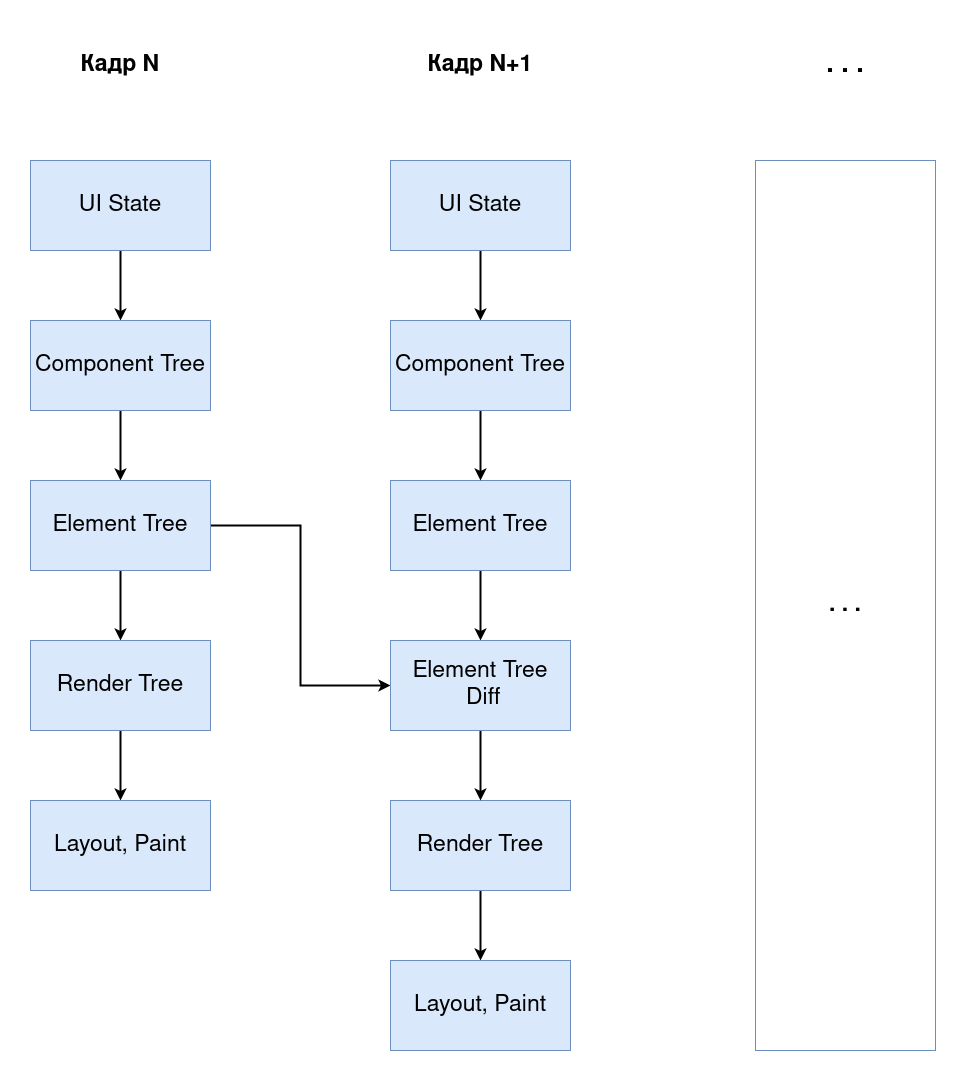
\includegraphics[width=\linewidth,height=0.9\linewidth,keepaspectratio]{resources/ui-render-pipeline.png}
\caption{Схематичный шаг алгоритма рендеринга пользовательского интерфейса}
\label{render-pipeline}
\end{figure}

Процесс отрисовки кадра \textit{N+1}, в свою очередь, повторяет
вышеописанный алгоритм за исключением следующего: дерево рендеринга
перестраивается на основании разницы между деревьями элементов текущего и
предыдущего кадров.
Подобное дополнение позволяет значительно повысить производительность
всего графического конвейера за счёт переиспользования вычислений,
хранящихся в дереве рендеринга предыдущего кадра.

\subsection{Существующие решения}

\subsection{Вывод}

\section{Архитектура и особенности реализации}
В данном разделе представлены архитектурные решения разрабатываемого языка и
и некоторые особенности их реализации.

\subsection{Архитектурные решения}
\label{section:architecture}
В ходе данной работы, выбор тех или иных архитектурных решений был
мотивирован удовлетворением итогового результата работы всем собранным
в главе~\ref{requirements-section} требованиям к спецификации и компилятору
современного языка разработки мобильных приложений.

\subsubsection{Встраивание  предметного языка в язык программирования \name{Accord}}
Язык разработки мобильных приложений является примером
предметно-ориентированного языка. В качестве способа реализации такого языка
был выбран метод встраивания предметного языка в базовый, которым является
язык \name{Accord}. Такое решение позволило переиспользовать существующий
прототип компилятора и спецификацию языка \name{Accord}, включая синтаксис,
синтаксический и семантический анализаторы, оптимизатор высокоуровневого
промежуточного представления, кодогенерации в \name{LLVM IR} и байткод
некоторой виртуальной машины.

Следствием этого решения является тот факт, что все синтаксические и
семантические конструкции и правила являются общими как для разработки
мобильных интерфейсов, так и для программ общего назначения. Другим
следствием является автоматическое соответствие решения таким требованиям,
как:
\begin{itemize}
	\item кроссплатформенная разработка: наличие кодогенерации в
	\name{LLVM IR} означает возможность потенциального запуска мобильных
	приложений, написанных на языке \name{Accord}, на всех платформах,
	поддерживаемых проектом \name{LLVM}~\cite{llvm-homepage}, а также
	на платформах, поддерживаемых виртуальной машиной, в байткод которой
	может быть оттранслирован исходный код приложения;
	\item предоставление отладочных возможностей: тот факт, что язык
	разработки мобильных приложений встроен в язык \name{Accord}, что
	означает их единство, гарантирует предоставление отладочных возможностей
	при разработке мобильных приложений в случае, если язык \name{Accord}
	имеет эти возможности. Несмотря на раннюю стадию разработки, язык
	\name{Accord} уже способен сохранять отладочную информацию о программе
	в формате \name{DWARF}~\cite{dwarf-homepage};
	\item поддержка интегрированной средой разработки: любая интегрированная
	среда разработки для языка \name{Accord} подходит и для разработки
	мобильных приложений на нём в силу единства языка разработки мобильных
	приложения и языка \name{Accord}.
\end{itemize}

Для достижения декларативности описания графического интерфейса в
спецификацию языка \name{Accord} были добавлены процедуры инициализации
объектов. На листинге~\ref{lst:accord-init} представлено упрощённое
синтаксическое правило определения процедур инициализации внутри
синтаксического контекста определения типа. Вызов процедуры инициализации
происходит автоматически при создании объекта во время выполнения программы.
Синтаксически данная семантика выглядит следующим образом:
\textit{TypeName(args)}, например, \textit{Text("This is an example")}.
\begin{lstlisting}[style=Antlr, caption=Синтаксическое правило процедур инициализации, label={lst:accord-init}]
INIT
	: 'init'
	;

type_init
	: INIT fn_params expression_sequence
	;
\end{lstlisting}

Для работы с реактивными данным в спецификацию языка \name{Accord} был
добавлен модификатор полей типов --- \textit{rx}. На данный момент, для
данных графической компоненты, помеченных модификатором \textit{rx},
компилятор автоматически генерирует функцию-мутатор. Задачей данной функции
является изменение реактивных данных и отметка необходимости обновления
графической компоненты, реактивные данные которой были изменены. В ходе
анализа графа потока управления, все изменения реактивных данных заменяются
на вызов сгенерированной функции-мутатора.
На листинге~\ref{lst:accord-rx-setter} представлен пример мутатора
реактивного поля \textit{counter} типа \textit{i32} компоненты
\textit{CounterComponent}.
\begin{lstlisting}[language=my_pseudo, caption=Пример функции-мутатора реактивных данных, label={lst:accord-rx-setter}]
fn CounterComponent.aco.set_counter(val: i32) {
    counter = val
    markNeedUpdate(this)
}
\end{lstlisting}
В дальнейшем семантика модификатора \textit{rx} будет расширена: он будет
применим не только к полям типов, но и к переменным. Изменение реактивных
данных будет приводить не только к обновлению графической комопненты на
экране, но и к обновлению других данных, как-либо использующих изменившиеся
реактивные данные.

\subsubsection{Статическая типизация графических компонент}
Различные графические компоненты могут сильно отличаться друг друга
семантически. Так, одни компоненты имеют динамическую
природу и могут изменяться от кадра к кадру, другие же --- статические ---
создаются лишь раз и не меняются на протяжении всей работы приложения.
Реальные графические компоненты, определяемые пользователем в приложении
могут быть достаточно сложными: включать большое количество различных
компонент, каждая из которых имеет своё собственное поведение и условия
обновления. Классический алгоритм обновления кадра, описанный
в главе~\ref{section:render-pipeline}, при условии поддержки компилятором,
использует статическую информацию о компонентах для минимизации
количества действий, необходимых для обновления кадра. Так, информация о
том, может ли компонента изменяться во время работы приложения, используется
средой времени исполнения для уменьшения количества сравнений
соответствующих компонент двух соседних кадров. Однако, знание таких
параметров, как тип и размер компоненты и её подкомпонент, а также
расположение подкомпонент относительно их родительской компоненты позволяет
избавиться от части операций, проводимых классическим алгоритмом во время
исполнения приложения ещё на этапе компиляции программы.

Рассмотрим пример графической компоненты на
листинге~\ref{lst:component-example}. Она представляет собой колонку,
состоящую из текста, кнопки и некоторой условной компоненты, которая
превращается в изображение или текст в зависимости от условия
\textit{condition}.
\begin{lstlisting}[language=my_pseudo, caption=Пример графической компоненты, label={lst:component-example}]
Column {
    Text("Current count: ${counter}")
    Button("Click on me!")
        .onClick(fn() { counter += 1 })
        .backgroundColor(Color.Green)
        .width(150px)
    ConditionalView(
        condition,
        Image("img.png"),
        Text("Empty")
    )
}
\end{lstlisting}
Зная статический тип данной компоненты
(листинг~\ref{lst:component-type-example}: $f0$ --- тип
под\-ком\-по\-ненты-колонки, $f1$ --- тип переменной \textit{counter}, $f2$
--- тип переменной \textit{condition}) и её представление в памяти
(рис.~\ref{component-layout-example}), компилятор способен ещё во время
компиляции приложения понять, какие компоненты могут быть изменены
во время работы приложения, а какие нет.
\begin{lstlisting}[escapeinside={(*}{*)}, caption=Пример статического типа компоненты, label={lst:component-type-example}]
struct {
    f0: Column[Text, Button, ConditionalView[Image, Text]]
    f1: i32
    f2: bool
}
\end{lstlisting}

\begin{figure}[H]
\centering
\MemoryLayout{
        32/blue!40/f0,
        40/green!40/f1,
        48/red!40/f2
}
\caption{Пример представления компоненты в памяти}
\label{component-layout-example}
\end{figure}
Имея представление компоненты в
памяти, компилятор может сгенерировать специализированную для конкретного
типа компоненты процедуру обновления
(листинг~\ref{lst:optimized-update-fn}). Эта процедура состоит из точечных
вызовов обновления только потенциально изменяемых во время работы приложения
компонент. Для сравнения такого подхода с классическим, введём понятия
некоторых условных операций, необходимых для обновления интерфейса согласно
главе~\ref{section:render-pipeline}. Пусть $A$ --- операция перехода между
узлами дерева компонент, $B$ --- проверка узла на изменяемость (проверка во
время исполнения программы), $C$ --- вызов процедуры обновления компоненты.
Тогда, если $N$ --- количество всех компонент, $M$ --- количество изменяемых
компонент, причём $M \leq N$, то для обновления одного кадра классическому
алгоритму необходимо произвести $(N - 1) * A + N * B + M * C$ операций,
в то время как описанному выше алгоритму лишь $M * C$.
\begin{lstlisting}[language=my_pseudo, caption=Пример сгенерированной процедуры обновления компоненты, label={lst:optimized-update-fn}]
fn Counter.rerender() {
    // skip Column
    Text.rerender(fieldAddress(0, 0), args...)
    // skip Button
    ConditionalView.rerender(
        fieldAddress(0, 2), args...,
    )
}
\end{lstlisting}
Для того, чтобы данная информация была доступна компилятору языка
\name{Accord}, в его спецификацию были добавлены синтаксис и семантика
наследования независимых типов (не имеющих типов-параметров) от
ненастроенных обобщённых типов с последующей автоматической настройкой
обобщённого типа-родителя в зависимости от содержимого определения
типа-потомка.

\subsection{Вывод}
Результатом выбора и реализации архитектурных решений, описанных в
пункте~\ref{section:architecture}, стало соответствие разработанного
решения всем требованиям, перечисленным в главе~\ref{requirements-section}.

\begin{appendices}
\section{Рекомендации по выбору подхода \newline  к созданию предметно-ориентирован-\\ного языка}
\label{appendixA}

\begin{figure}[h]
\centering
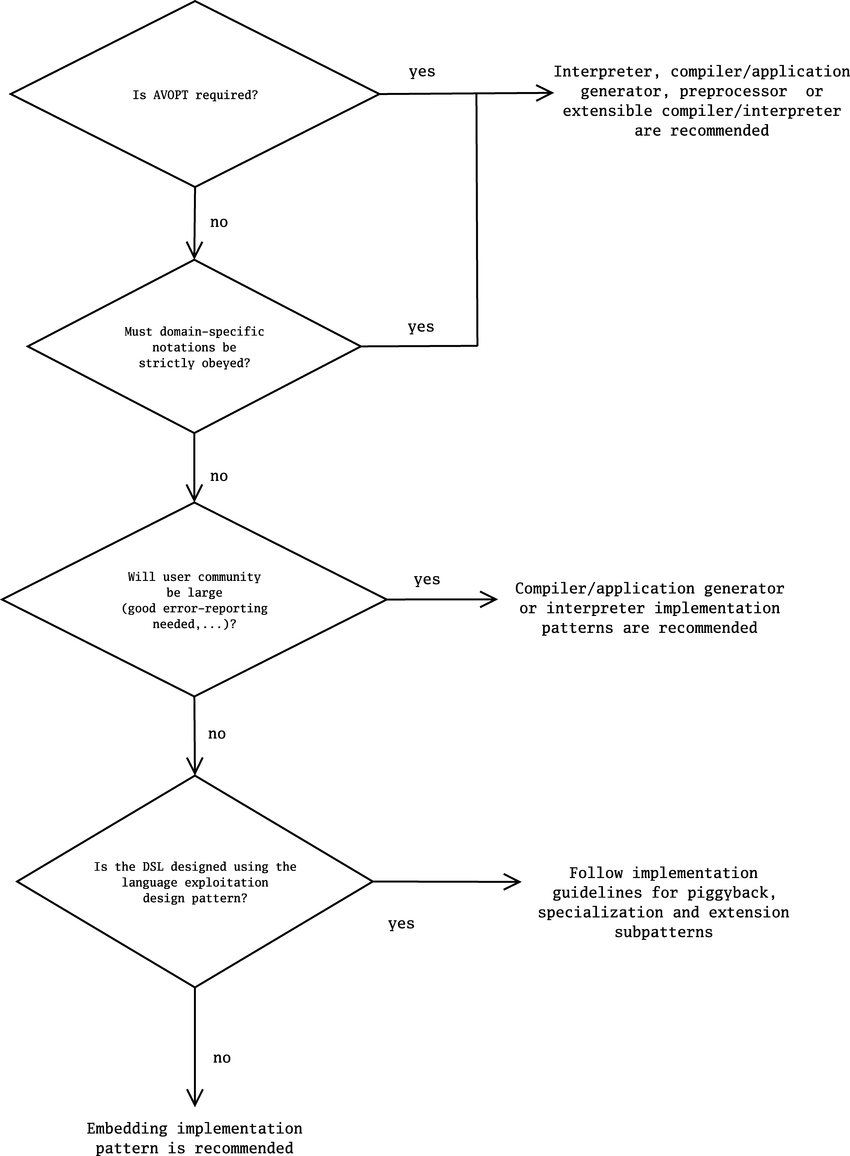
\includegraphics[width=\linewidth,height=1.1\linewidth,keepaspectratio]{resources/dsl-implementation-guideline.png}
\caption{Алгоритм выбора метода разработки DSL~\cite{when-and-how-develop-dsl}}
\end{figure}

\end{appendices}



\setmonofont[Mapping=tex-text]{CMU Typewriter Text}
\nocite{*}
\bibliographystyle{ugost2008ls}
\bibliography{diploma.bib}
\end{document}